\documentclass[border=10pt]{standalone}
\usepackage{xcolor}
\usepackage{pgfplots}
\usepackage{tikz}
\begin{document}
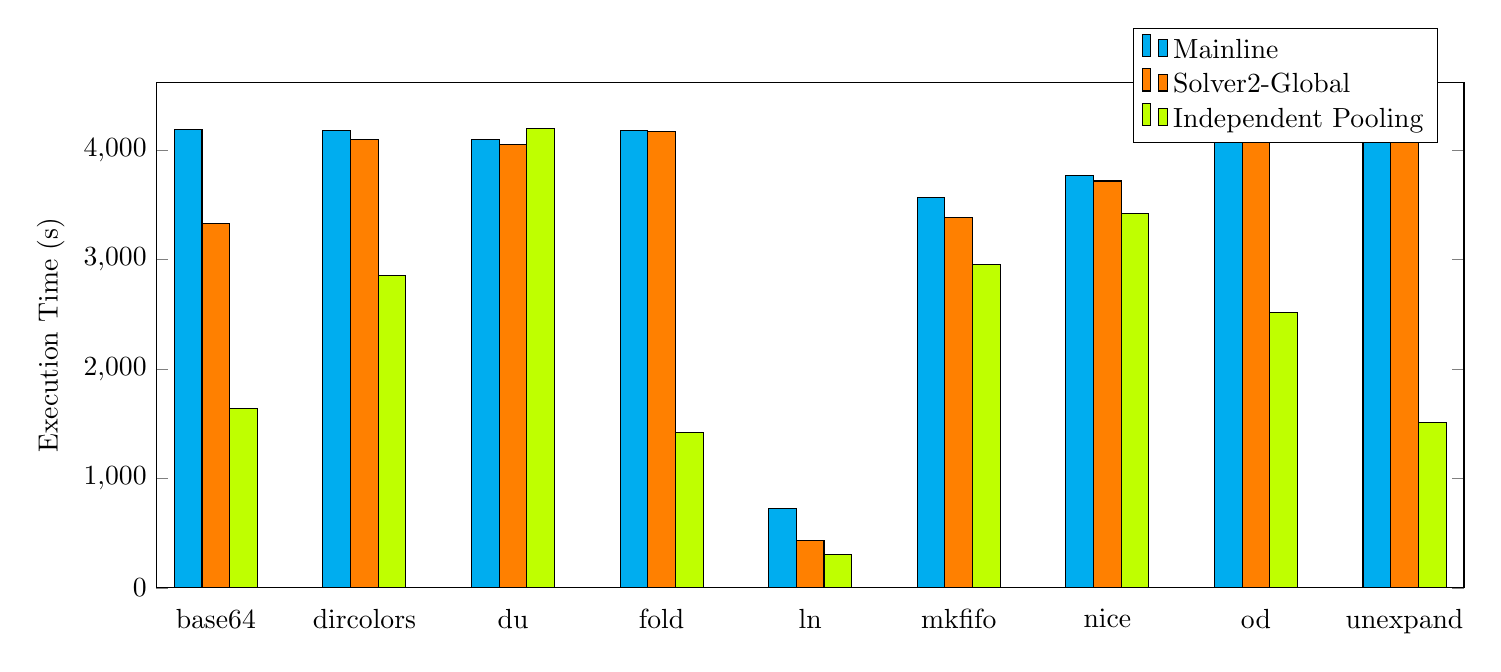
\begin{tikzpicture}
    \begin{axis}[
            width  = 1.5 * \textwidth,
            height = 8cm,
            major x tick style = transparent,
            % tickwidth=10,
            ybar=0,
            bar width=10pt,
            % ymajorgrids = true,
            ylabel = {Execution Time (s)},
            symbolic x coords={base64,dircolors,du,fold,ln,mkfifo,nice,od,unexpand},
            xtick = data,
            scaled y ticks = false,
            enlarge x limits=0.05,
            ymin=0,
            legend cell align=left,
            legend style={
                    at={(0.98,0.88)},
                    anchor=south east,
                    % column sep=1ex
                }
        ]
        \addplot[style={cyan,fill=cyan,mark=none}, draw=black]
        coordinates {(base64,4183.76) (dircolors,4176.50) (du,4094.84) (fold,4178.14) (ln,727.92) (mkfifo,3563.66) (nice,3765.43) (od,4070.13) (unexpand,4191.03)};
        \addplot[style={orange,fill=orange,mark=none}, draw=black]
        coordinates {(base64,3323.54) (dircolors,4096.28) (du,4051.29) (fold,4171.08) (ln,433.45) (mkfifo,3385.87) (nice,3715.43) (od,4133.98) (unexpand,4193.22)};
        \addplot[style={lime,fill=lime,mark=none}, draw=black]
        coordinates {(base64,1640.25) (dircolors,2853.77) (du,4195.09) (fold,1422.00) (ln,306.35) (mkfifo,2956.52) (nice,3419.83) (od,2513.96) (unexpand,1513.60)};

        \legend{Mainline,Solver2-Global,Independent Pooling}
    \end{axis}
\end{tikzpicture}
\end{document}
